\section{Design}
\label{sec:design}

% Around 5 pages about functional aspects of the FeedApp application.
The main purpose of the FeedApp is to deliver a modern web application that offers a seamless and intuitive experience, allowing users to log in, craft their own surveys and cast votes on existing polls.

\subsection{Use cases}
 \textbf{User Authentication and Authorization}:
In FeedApp, user authentication and authorization are handled using OAuth 2.0 to make logging in secure and easy. When users want to log in, they can either use their FeedApp credentials or sign in through a trusted service like Google. If they choose a third-party login, they are redirected to that provider to confirm their identity. Once they’re logged in, the system gives them a token that lets them interact with the app without having to log in again for every action. This keeps things secure and makes the whole experience smoother for the user.
\medskip

\noindent
 \textbf{Survey Creation}:
One of the main features of FeedApp is letting users create surveys. After logging in, users can go to the "Create Survey" page to start building their survey. First, they give the survey a title. Then they can add multiple polls to it, setting the order of each poll so that everything flows the way they want. Inside each poll, they can add as many options as needed for participants to choose from. Once the user is done creating their survey, it gets saved in the system and is ready for others to participate in. This makes it simple to create detailed surveys with multiple questions and options.
\medskip

\noindent
 \textbf{Voting on polls}:
Voting is another important part of FeedApp. Logged-in users can find active surveys, go through the polls, and select the options they want to vote for. Once they’ve made their choices, they submit their votes, and the system processes them. After the vote is recorded, the results are updated in real time so everyone can see the latest vote counts. This real-time feature makes the app more interactive and lets participants stay up-to-date on how the survey is doing.
\medskip

\noindent
 \textbf{View Survey Results}:
FeedApp also makes it easy to view survey results, both for the person who created the survey and for the people who participated in it. After a survey is published, users can look at the results for each poll. The app shows things like the total number of votes and how the votes are spread across the different options. These results update automatically whenever new votes are added, so the data is always current. This feature helps creators see how their surveys are performing and gives participants a clear view of the outcome.

\begin{figure}[thb]
	\centering
	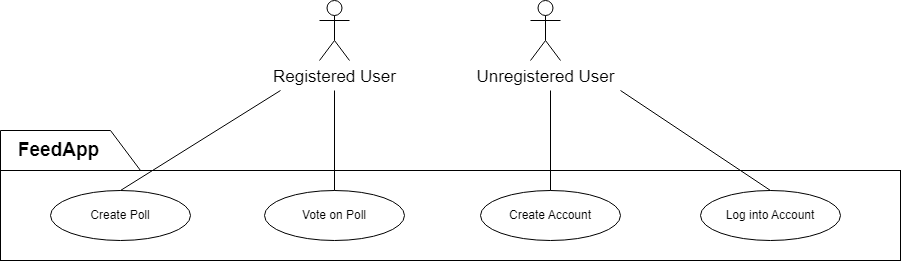
\includegraphics[scale=0.5]{figs/usecase.png}
	\caption{Use Case}
	\label{fig:usecase}
\end{figure}

\subsection{Domain model}
\begin{figure}[!htbp]
	\centering
	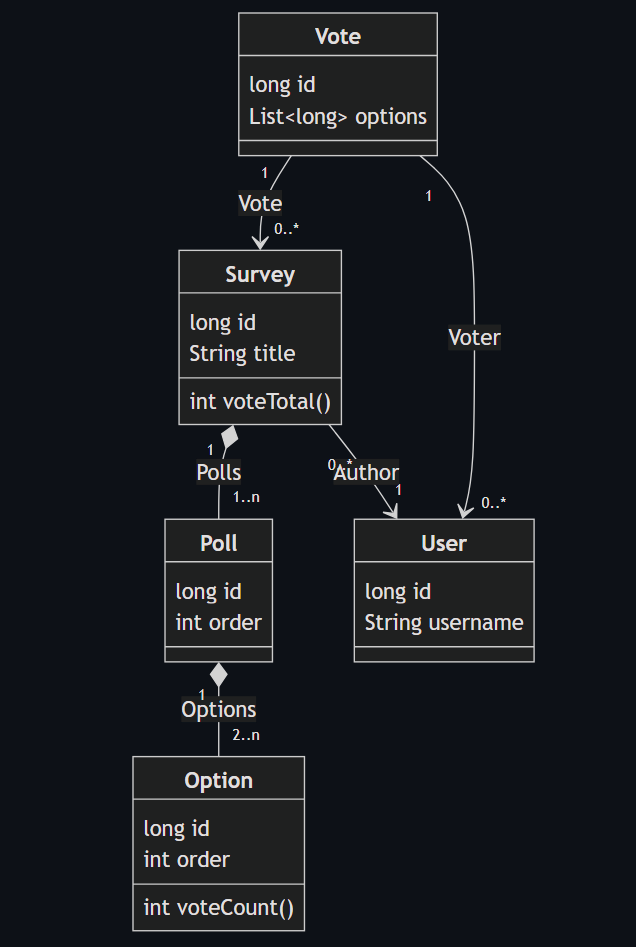
\includegraphics[scale=0.5]{figs/domainmodel.png}
	\caption{The Domain Model.}
	\label{fig:domainmodel}
\end{figure}
The domain model for the FeedApp application captures the core entities and their relationships, providing the foundation for managing surveys, polls, and user interactions. This model ensures a structured and scalable approach to data representation, supporting the application's primary functions such as survey creation, voting, and user management.
\medskip

\subsubsection*{Entities in the Domain Model}

The following entitites can be seen in figure~\ref{fig:domainmodel}:
\smallskip

\noindent
 \textbf{User}:
A User represents an individual interacting with the system, either as a participant in surveys or as an author creating new polls. The Survey entity acts as the central object, representing a collection of polls authored by a user. Each survey is comprised of one or more Polls, which in turn consist of multiple Options that users can select from when casting their votes. The Vote entity captures the act of participation, linking users with the options they select in a given poll.
\medskip

\noindent
 \textbf{Survey}:
A Survey is the primary container entity, representing a collection of polls authored by a user. Each survey has a unique id and a title describing its purpose. The voteTotal() method calculates the total number of votes across all associated polls, providing a quick summary of survey engagement.
\medskip

\noindent
 \textbf{Poll}:
The Poll entity is a component of a survey, representing a single voting instance within it. Polls are ordered using the order attribute, ensuring that their sequence within a survey can be maintained. Each poll is linked to multiple options, allowing users to select from predefined choices.
\medskip

\noindent
 \textbf{Option}:
Options are individual choices within a poll. Each option is uniquely identified by an id and has an associated order attribute to define its position within the poll. The voteCount() method calculates the number of votes an option has received, enabling detailed poll result analysis.
\medskip

\noindent
 \textbf{Vote}:
The Vote entity captures user participation in polls. A vote links a user to specific survey options they have chosen, ensuring accurate representation of voting behavior. The entity includes a unique id and relationships with the User, Survey, and Option entities.
\medskip

\noindent
\subsubsection*{Relationships}
\noindent
The relationships between these entities are key to the domain model's functionality. A survey can have many polls, and each poll must have at least two options to be valid. Votes are associated with both users and surveys, reflecting the choices made by participants. This model not only reflects the application's functional requirements but also ensures data integrity through these defined relationships. Additionally, the use of attributes such as timestamps and unique identifiers allows for detailed analytics and user tracking, which are essential for the platform's growth and adaptability.
\medskip

\noindent
This domain model provides a solid foundation for implementing the core features of FeedApp, including survey creation, user participation, and vote aggregation. Its design ensures that the application can scale to accommodate a growing number of users and complex interactions, while maintaining a clear and manageable structure.

\subsection{Architecture}
\begin{figure}[!htbp]
	\centering
	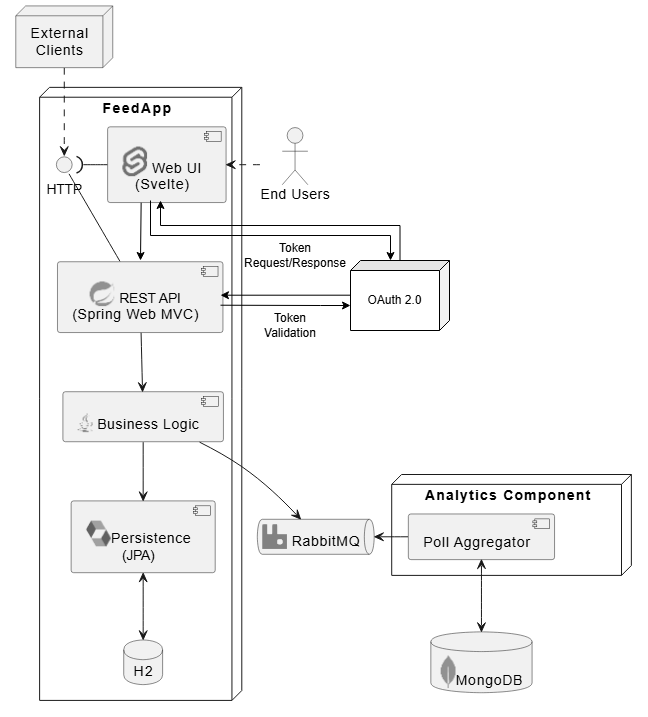
\includegraphics[scale=0.5]{figs/architecture.png}
	\caption{Architecture}
	\label{fig:architecture}
\end{figure}

The architecture of FeedApp, shown in Figure~\ref{fig:architecture}, follows a modular, layered design. It includes a frontend, backend, and supporting infrastructure, all working together to provide a secure and scalable application.

The frontend, built with Svelte, offers users a fast and responsive interface for interacting with surveys. This Single Page Application (SPA) communicates with the backend using HTTP requests and includes OAuth 2.0 token-based authentication to keep interactions secure.

The backend is implemented using Spring Boot. It provides a RESTful API through Spring Web MVC, which handles requests from the frontend and coordinates with the business logic and persistence layers. Core functionalities, such as survey and vote management, are handled in this layer.

The persistence layer uses both PostgreSQL and MongoDB. PostgreSQL stores structured data like users, surveys, polls, and votes, ensuring data consistency. MongoDB handles unstructured or semi-structured data, such as analytics and logs, allowing flexible queries.

RabbitMQ, a message broker, enables communication between components and supports asynchronous tasks like vote aggregation. This design ensures the system can handle high loads efficiently.

Security is a core focus, with OAuth 2.0 providing robust user authentication and authorization. Tokens issued by an external or custom Authorization Server are used to validate user identities and enforce access controls.

This layered design makes FeedApp modular, easy to maintain, and scalable. It is well-suited for the current requirements and provides a strong foundation for future improvements.



%%%%
\subsubsection{OAuth 2.0: How It Works (Google Implementation)}
OAuth 2.0 is a framework that allows secure access to user resources without exposing their credentials. It is widely used for authenticating users and authorizing API calls, and Google’s implementation is one of the most commonly used examples.

Figure~\ref{fig:oauth2-google} illustrates the sequence of interactions in an OAuth 2.0 flow, specifically using Google's implementation. Here's a step-by-step explanation of the process:
\begin{enumerate}
\item \textbf{Request Token}:
The user begins by interacting with the FeedApp (referred to as "Your JS App" in the figure) and initiates the login process. The application sends a request to Google’s servers to obtain an authorization token.

\item \textbf{User Login and Consent}:
Google then prompts the user to log in and provide consent for the requested scopes (permissions). These scopes define what the application is allowed to access on the user's behalf, such as their profile or email address.

\item \textbf{Token Response}:
Once the user consents, Google generates and returns an Access Token to the application. This token represents the user’s identity and their permissions.

\item \textbf{Validate Token}:
Before making API requests, the application can validate the token with Google’s servers to ensure it is legitimate and has not expired. This step ensures an additional layer of security.

\item \textbf{Use Token to Call Google API}:
After validation, the application can use the token to securely call Google’s APIs or perform other operations. The token is included in the Authorization header of API requests.
\end{enumerate}

This flow highlights the key advantage of OAuth 2.0: the user's credentials are never directly shared with the application, reducing security risks. Instead, a short-lived token is used, which can be revoked or scoped as needed \cite{google:oauth}.

\begin{figure}[htbp]
\centering
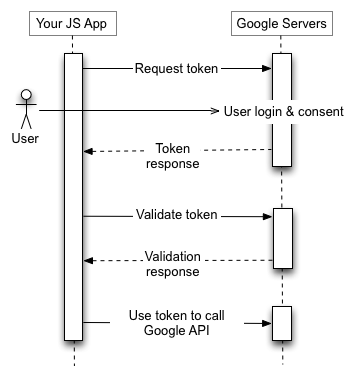
\includegraphics[scale=0.5]{figs/OAuthGoogle.png}
\caption{OAuth 2.0 Flow with Google Implementation.}
\label{fig:oauth2-google}
\end{figure}

Security and Benefits
OAuth 2.0's token-based approach is highly secure, as tokens can be limited in scope and validity. Google’s implementation also ensures strong user consent flows, making it suitable for applications requiring sensitive data access. For FeedApp, this implementation guarantees that only authenticated and authorized users can create surveys, cast votes, and access results.

This explanation is based on official documentation from Google Developers, which provides further detai

